% \iffalse
\let\negmedspace\undefined
\let\negthickspace\undefined
\documentclass[journal,12pt,twocolumn]{IEEEtran}
\usepackage{cite}
\usepackage{amsmath,amssymb,amsfonts,amsthm}
\usepackage{algorithmic}
\usepackage{graphicx}
\usepackage{textcomp}
\usepackage{xcolor}
\usepackage{txfonts}
\usepackage{listings}
\usepackage{enumitem}
\usepackage{mathtools}
\usepackage{gensymb}
\usepackage{comment}
\usepackage[breaklinks=true]{hyperref}
\usepackage{tkz-euclide} 
\usepackage{listings}
\usepackage{gvv}                                        
\def\inputGnumericTable{}                                 
\usepackage[latin1]{inputenc}                                
\usepackage{color}                                            
\usepackage{array}                                            
\usepackage{longtable}                                       
\usepackage{calc}                                             
\usepackage{multirow}                                         
\usepackage{hhline}                                           
\usepackage{ifthen}                                           
\usepackage{lscape}
\newtheorem{theorem}{Theorem}[section]
\newtheorem{problem}{Problem}
\newtheorem{proposition}{Proposition}[section]
\newtheorem{lemma}{Lemma}[section]
\newtheorem{corollary}[theorem]{Corollary}
\newtheorem{example}{Example}[section]
\newtheorem{definition}[problem]{Definition}
\newcommand{\BEQA}{\begin{eqnarray}}
\newcommand{\EEQA}{\end{eqnarray}}
\newcommand{\define}{\stackrel{\triangle}{=}}
\theoremstyle{remark}

\newtheorem{rem}{Remark}
\begin{document}
\parindent 0px
\bibliographystyle{IEEEtran}
\title{Assignment 10.5.3\_13Q}
\author{EE23BTECH11219 - Rada Sai Sujan$^{}$% <-this % stops a space
}
\maketitle
\newpage
\bigskip
\section*{Question}
Find the sum of the first 15 multiples of 8. \\
\solution

    \begin{figure}[ht]
        \centering
        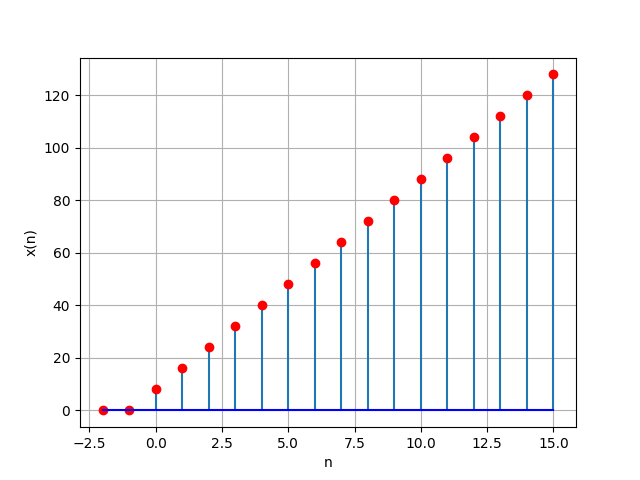
\includegraphics[width=\columnwidth]{figs/a.png}
        \caption{Plot of x(n) $vs$ n}
        \label{fig:10.5.3.13.1}
    \end{figure}
The $Z$-transform of p\brak n is defined as 
\begin{align}
    P\brak Z=\sum\limits_{n=-\infty}^{\infty}p\brak nz^{-n}         \label{eq:10.5.3.13.1}
\end{align}
\begin{align}
    u\brak{n} \system{Z} U\brak{x}&=\dfrac{1}{(1-{z}^{-1})}, \,\,\,|z|>1 \label{eq:10.5.3.13.2}
\end{align}
From \eqref{eq:10.5.3.13.1} and \eqref{eq:10.5.3.13.2}
\begin{align}
    U(Z)&=\sum\limits_{-\infty}^{\infty}u(n)z^{-n}   \\
    \Rightarrow \dfrac{d(U(z))}{dz} &= -z^{-1}\sum\limits_{n=-\infty}^{\infty}-nu\brak nz^{-n}   
\end{align}
\begin{align}
    \therefore nu\brak{n} \system{Z} \dfrac{z^{-1}}{{(1-z^{-1})}^2}, \,\,\,|z|>1
\end{align}
For an AP,
\begin{align}
    x\brak n &=[ x\brak 0 + nd ]u\brak n    \\
    x\brak n&=8n+8  \\
    \Rightarrow X\brak Z &= \dfrac{x\brak 0}{1-z^{-1}} + \dfrac{dz^{-1}}{{(1-z^{-1})}^{2}}, \,\,\,|z|>1 
\end{align}
\begin{align}
    y\brak{n}&=x\brak{n}\ast u\brak{n}\\
    Y\brak{z}&=X\brak{z}U\brak{z}
\end{align}
\begin{align}
    Y\brak{z}&=\brak{\dfrac{x(0)}{1-z^{-1}} + \dfrac{dz^{-1}}{(1-z^{-1})^{2}}}\brak{\dfrac{1}{1-z^{-1}}}\\
    &n^2u(n)\system{Z} \dfrac{z^{-1}+z^{-2}}{(1-z^-1)^3}
 \end{align}
 By performing inverse $Z$-transform on Y\brak{z}
\begin{align}
    y\brak{n}&=x\brak{0}\brak{n+1}u\brak{n}+d\brak{\dfrac{{n\brak{n+1}}}{2}}u\brak{n}   \\
    y\brak{n}&=\dfrac{n+1}{2}\brak{2x\brak{0}+nd}   \\
    y\brak n &= \dfrac{15}{2}\brak {16+120}    \\
    y\brak n &=960
 \end{align}
\begin{table}[htbp]
    \def\arraystretch{1.5}
    \centering
    \begin{tabular}{|p{2.3cm}|p{2.3cm}|p{2.3cm}|}
    \hline
    PARAMETER & VALUE & DESCRIPTION \\ \hline
    x\brak0 & 8 & First term \\ \hline
    n & 15 & Number of terms \\ \hline
    d & 8 & common difference \\ \hline
    S &960 & Sum of n terms \\ \hline
    \end{tabular}
    \caption{Parameter Table1}
    \label{tab:1}
\end{table}

\end{document}
